\documentclass[12pt]{article}

\usepackage{amsmath}
\usepackage{array}
\usepackage{caption}
\usepackage[top=1in, bottom=1in, left=0.75in, right=0.75in]{geometry}
\usepackage{graphicx}
\usepackage[colorlinks=true, allcolors=blue]{hyperref}
\usepackage[utf8]{inputenc}
\usepackage{minted}
\usepackage{multirow}
\usepackage{nameref}
\usepackage{pdfpages}
\usepackage[section]{placeins}

\graphicspath{{figures/}}

\begin{document}

\begin{titlepage}
  \begin{center} \LARGE
    \vspace*{1.5in}

    ECE 272 Lab 4

    Fall 2018

    \vfill

    SystemVerilog and Complex Projects

    Phi Luu

    \vfill

    October 31\textsuperscript{st}, 2018

    Grading TA: Edgar Perez

    Lab Partner: Benjamin Geyer

    \vspace{1.5in}
  \end{center}
\end{titlepage}

%%%%%%%%%%%%%%%%%%%%%%%%%%%%%%%%%%%%%%%%%%%%%%%%%%%%%%%%%%%%%%%%%%%%%%%%%%%%%%%%
% Introduction
%%%%%%%%%%%%%%%%%%%%%%%%%%%%%%%%%%%%%%%%%%%%%%%%%%%%%%%%%%%%%%%%%%%%%%%%%%%%%%%%
\section{Introduction}

This lab focuses on implementing combinational logic using a hardware description language (HDL) called SystemVerilog. SystemVerilog uses text to define the specifications of a system. Although it is not as intuitive as describing a system with a schematic (like labs 1, 2, and 3), SystemVerilog allows the users to design more complex systems in a simpler way, especially for sequential circuits.

A simple SystemVerilog-schematic comparison can be seen in a two-input AND gate example in Figure~\ref{figure:1} below:

\begin{figure}[ht]
  \centering
  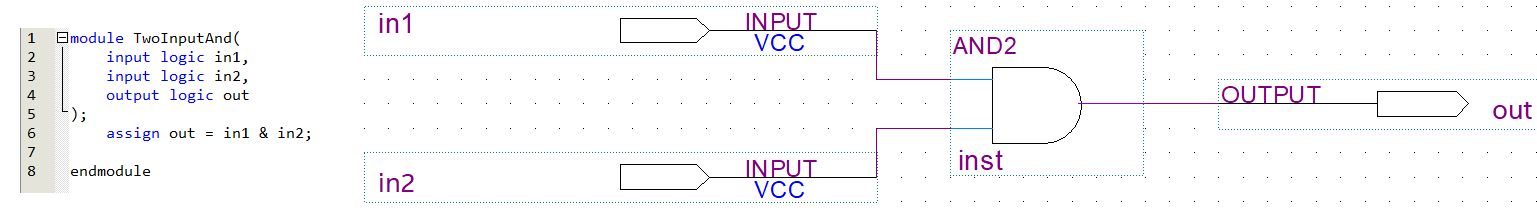
\includegraphics[width=\textwidth]{systemverilog_schematic_comparison.png}
  \caption{A high-accuracy-demand process of drawing a schematic can be simplified into 8 lines of SystemVerilog text file}
  \label{figure:1}
\end{figure}

During this lab, I and Ben design a seven-segment display counter and multiplier. We use 10 switches from the FPGA to represents 10-bit binary numbers, multiply them with a constant according to the input push buttons, and decode the digits to 6 seven-segment displays.

%%%%%%%%%%%%%%%%%%%%%%%%%%%%%%%%%%%%%%%%%%%%%%%%%%%%%%%%%%%%%%%%%%%%%%%%%%%%%%%%
% Design
%%%%%%%%%%%%%%%%%%%%%%%%%%%%%%%%%%%%%%%%%%%%%%%%%%%%%%%%%%%%%%%%%%%%%%%%%%%%%%%%
\section{Design}

We use all 10 switches of the FPGA to represent a 10-bit binary input and 6 seven-segment displays to represent a 6-digit decimal output. To produce the output from the inputs, we implement a 12:17 multiplexer which takes the 10-bit input of the switches as the multiplicand and 2-bit push buttons as the multiplier. The output of the multiplexer is expressed as a 17-bit binary. Next, we parse that output into a parser to split the 17-bit binary into 6 groups of 4-bit binary numbers. Each group of 4-bit binary numbers will then go to a seven-segment display decoder and produce the corresponding digit. Intuitively, the system is illustrated as in Figure~\ref{figure:2} below:

\begin{figure}[ht]
  \centering
  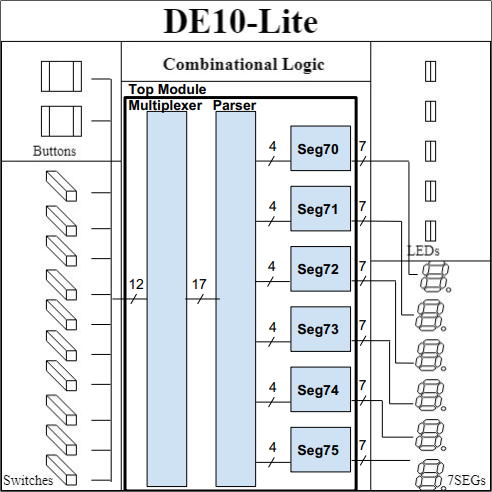
\includegraphics[width=0.6\textwidth]{lab4_block_diagram.png}
  \caption{Block diagram}
  \label{figure:2}
\end{figure}

Since the LEDs in the seven-segment displays are active-low, the output signal needs to be LOW (or $0$) to activate the LEDs and to be HIGH (or $1$) to deactivate the LEDs. Table~\ref{table:1} decodes a decimal number into a binary number and then to the signal in a seven-segment display.

\begin{table}[ht]
  \centering
  \begin{tabular}{ | c | c | c | c | c | c | c | c | c | }
  \hline
  \textbf{Decimal}                                                       & \textbf{Binary}                                                         & \textbf{Seg\textsubscript{A}} & \textbf{Seg\textsubscript{B}} & \textbf{Seg\textsubscript{C}} & \textbf{Seg\textsubscript{D}} & \textbf{Seg\textsubscript{E}} & \textbf{Seg\textsubscript{F}} & \textbf{Seg\textsubscript{G}} \\ \hline
  0                                                                      & 0000                                                                    & 0                             & 0                             & 0                             & 0                             & 0                             & 0                             & 1                             \\ \hline
  1                                                                      & 0001                                                                    & 1                             & 0                             & 0                             & 1                             & 1                             & 1                             & 1                             \\ \hline
  2                                                                      & 0010                                                                    & 0                             & 0                             & 1                             & 0                             & 0                             & 1                             & 0                             \\ \hline
  3                                                                      & 0011                                                                    & 0                             & 0                             & 0                             & 0                             & 1                             & 1                             & 0                             \\ \hline
  4                                                                      & 0100                                                                    & 1                             & 0                             & 0                             & 1                             & 1                             & 0                             & 0                             \\ \hline
  5                                                                      & 0101                                                                    & 0                             & 1                             & 0                             & 0                             & 1                             & 0                             & 0                             \\ \hline
  6                                                                      & 0110                                                                    & 0                             & 1                             & 0                             & 0                             & 0                             & 0                             & 0                             \\ \hline
  7                                                                      & 0111                                                                    & 0                             & 0                             & 0                             & 1                             & 1                             & 1                             & 1                             \\ \hline
  8                                                                      & 1000                                                                    & 0                             & 0                             & 0                             & 0                             & 0                             & 0                             & 0                             \\ \hline
  9                                                                      & 1001                                                                    & 0                             & 0                             & 0                             & 0                             & 1                             & 0                             & 0                             \\ \hline
  \end{tabular}
  \caption{Conversion table between decimal, 4-bit binary, and seven-segment signals}
  \label{table:1}
\end{table}

\newpage

When we implemented a seven-segment display decoder in lab 3, we had to use Karnaugh maps to simplify Boolean equations. We also had to spend a lot of time connecting visual elements on the schematic of Quartus Prime. In this lab, however, we only need to type descriptions of the hardware into SystemVerilog files, and the compiler will take care of the rest. This feature will be quite convenient when we design highly complex circuits in the future.

Because we don't draw any schematic in this lab, we write SystemVerilog code that describes the connections between the elements in the circuit. The source code can be found in the \nameref{section:Appendix} section at the end of this report.

We designate the switch at the corner of the FPGA as bit $0$ of the Switches array in our SystemVerilog code (the switch labeled as \textit{SW0} on the board) and so on. We designate the seven-segment display nearest to the switches as Seg70 (the display labeled \textit{HEX0} on the board). Finally, we designate the push button further from the switches as bit $0$ of the Buttons array in our SystemVerilog code (the button labeled \textit{KEY0} on the board). See the \nameref{section:Appendix} for more details.

%%%%%%%%%%%%%%%%%%%%%%%%%%%%%%%%%%%%%%%%%%%%%%%%%%%%%%%%%%%%%%%%%%%%%%%%%%%%%%%%
% Results
%%%%%%%%%%%%%%%%%%%%%%%%%%%%%%%%%%%%%%%%%%%%%%%%%%%%%%%%%%%%%%%%%%%%%%%%%%%%%%%%
\section{Results}

We compile and simulate the project on ModelSim and obtain the following waveforms:

\begin{figure}[ht]
  \centering
  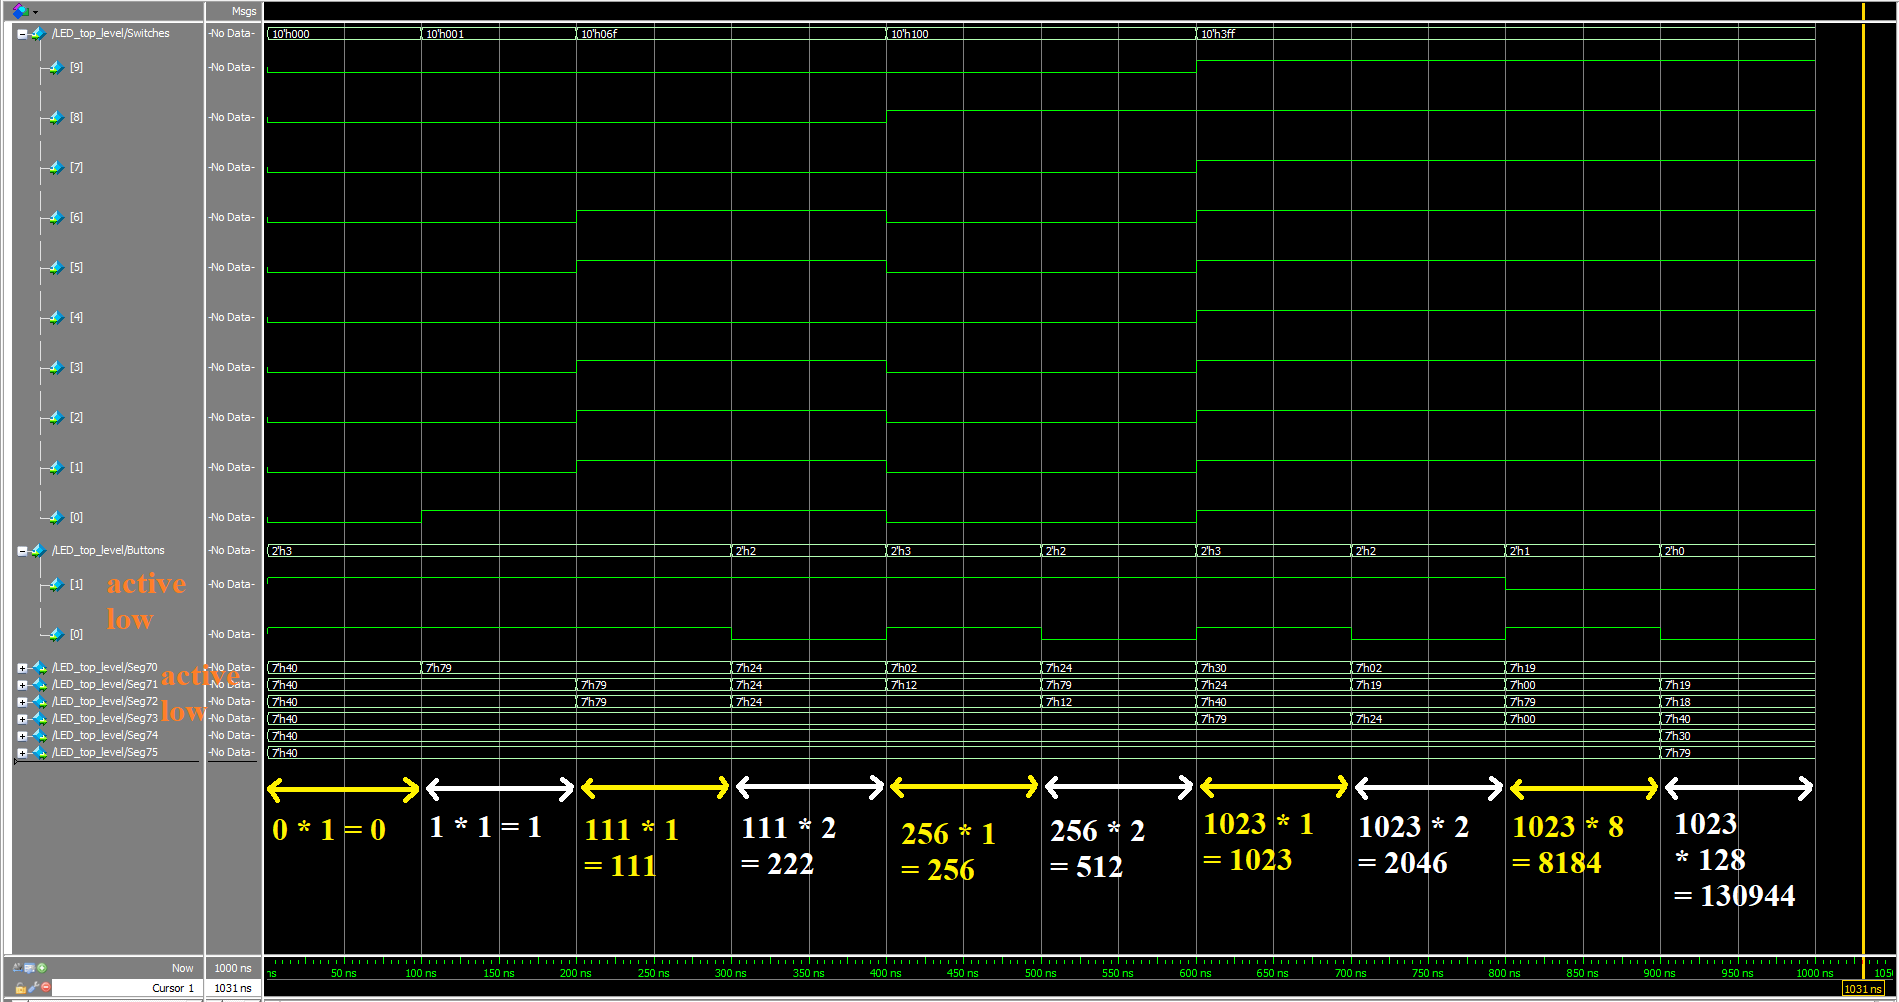
\includegraphics[width=\textwidth]{lab4_simulation.png}
  \caption{Simulation waveform of a few test examples. \href{https://i.imgur.com/1UjCN6E.png}{High-resolution image}}
  \label{figure:3}
\end{figure}

\newpage

Each 100-ns interval (2 columns) is a test case. Each of the test cases' inputs and output are specified with a two-way arrow. For example, from 100 ns to 200 ns (from the third column to the fourth column), the switch input is equivalent to a $1$ in decimal system (\textit{SW1} turned on and all other switches turned off), and the button input is equivalent to a $1$ in decimal system (all buttons not pressed), and the output of all 6 seven-segment displays is $000001$ (reading from $\text{Seg75}$ to $\text{Seg70}$).

Using the same method, we obtain the result of all test cases. Since the results are consistent with mathematical calculations, we believe the simulation of the project is a success.

Finally, we upload the project to the real FPGA. We do thorough tests on the real board, and the results are consistent with the simulations as well as mathematical laws. Therefore, we have successfully implemented a seven-segment display decoders with a multiplexer and a parser using SystemVerilog.

%%%%%%%%%%%%%%%%%%%%%%%%%%%%%%%%%%%%%%%%%%%%%%%%%%%%%%%%%%%%%%%%%%%%%%%%%%%%%%%%
% Experiment Notes
%%%%%%%%%%%%%%%%%%%%%%%%%%%%%%%%%%%%%%%%%%%%%%%%%%%%%%%%%%%%%%%%%%%%%%%%%%%%%%%%
\section{Experiment Notes}

%%%%%%%%%%%%%%%%%%%%%%%%%%%%%%%%%%%%%%%%
% Reflection
%%%%%%%%%%%%%%%%%%%%%%%%%%%%%%%%%%%%%%%%
\subsection*{Reflection}

It took me approximately 20 minutes to get used to writing SystemVerilog on Quartus Prime. The combinational logic portion of the project was quite easy. I started to prefer writing SystemVerilog to sketching schematic because I could simplify tedious graphic circuit contruction using a few lines in a \textit{case} block of SystemVerilog.

I think this lab was an easy yet a necessary lab for students to become more familiar with SystemVerilog and how to use HDL to "write" circuits. I plan to program circuits in SystemVerilog from now on because it is more consistent than wiring the components in a graphical interface.

%%%%%%%%%%%%%%%%%%%%%%%%%%%%%%%%%%%%%%%%
% Study Questions
%%%%%%%%%%%%%%%%%%%%%%%%%%%%%%%%%%%%%%%%
\subsection*{Study Questions}

\begin{enumerate}
  \item Describe how to control a 7-seg display using a state machine and lighting each digit one at a time.

  To control a single seven-segment display which displays decimal digits, a 10-state state machine is needed---each state for every decimal digit. Let S0 be the state corresponding to the decimal digit 0, S1 be the state corresponding to decimal digit 1, and so on. Since the FSM lights each digit one at a time, using this structure, Table~\ref{table:2} is constructed as the state transition table:

  \begin{table}[ht]
    \centering
    \begin{tabular}{|c|c|}
    \hline
    \textbf{\begin{tabular}[c]{@{}c@{}}Current State\\ S\end{tabular}} & \textbf{\begin{tabular}[c]{@{}c@{}}Next State\\ S'\end{tabular}} \\ \hline
    S0                                                                 & S1                                                               \\ \hline
    S1                                                                 & S2                                                               \\ \hline
    S2                                                                 & S3                                                               \\ \hline
    S3                                                                 & S4                                                               \\ \hline
    S4                                                                 & S5                                                               \\ \hline
    S5                                                                 & S6                                                               \\ \hline
    S6                                                                 & S7                                                               \\ \hline
    S7                                                                 & S8                                                               \\ \hline
    S8                                                                 & S9                                                               \\ \hline
    S9                                                                 & S0                                                               \\ \hline
    \end{tabular}
    \caption{State transition table of a 7-seg FSM}
    \label{table:2}
  \end{table}

  10 states are encoded into 4-bit binary numbers, as follows:

  \begin{table}[ht]
    \centering
    \begin{tabular}{ | c | c | }
    \hline
    \textbf{State} & \textbf{Encoding} $\mathbf{S_{3:0}}$ \\ \hline
    S0             & 0000                                 \\ \hline
    S1             & 0001                                 \\ \hline
    S2             & 0010                                 \\ \hline
    S3             & 0011                                 \\ \hline
    S4             & 0100                                 \\ \hline
    S5             & 0101                                 \\ \hline
    S6             & 0110                                 \\ \hline
    S7             & 0111                                 \\ \hline
    S8             & 1000                                 \\ \hline
    S9             & 1001                                 \\ \hline
    \end{tabular}
    \caption{State binary encoding of a 7-seg display FSM}
    \label{table:3}
  \end{table}

  Using Table~\ref{table:1} as a binary-to-seven-segment conversion table, the state transition table with binary encodings and outputs is constructed in Table~\ref{table:4} below:

  \begin{table}[ht]
    \centering
    \begin{tabular}{ | c | c | c | c || c | c | c | c | c | c | c || c | c | c | c | }
    \hline
    \multicolumn{4}{|c||}{\textbf{Current State}}                     & \multicolumn{7}{c||}{\textbf{Outputs}}                                                                                                                                                            & \multicolumn{4}{c|}{\textbf{Next State}}                              \\ \hline
    $\mathbf{S_3}$ & $\mathbf{S_2}$ & $\mathbf{S_1}$ & $\mathbf{S_0}$ & $\mathbf{\textbf{Seg}_G}$ & $\mathbf{\textbf{Seg}_F}$ & $\mathbf{\textbf{Seg}_E}$ & $\mathbf{\textbf{Seg}_D}$ & $\mathbf{\textbf{Seg}_C}$ & $\mathbf{\textbf{Seg}_B}$ & $\mathbf{\textbf{Seg}_A}$ & $\mathbf{S'_3}$ & $\mathbf{S'_2}$ & $\mathbf{S'_1}$ & $\mathbf{S'_0}$ \\ \hline
    0              & 0              & 0              & 0              & 1                         & 0                         & 0                         & 0                         & 0                         & 0                         & 0                         & 0               & 0               & 0               & 1               \\ \hline
    0              & 0              & 0              & 1              & 1                         & 1                         & 1                         & 1                         & 0                         & 0                         & 1                         & 0               & 0               & 1               & 0               \\ \hline
    0              & 0              & 1              & 0              & 0                         & 1                         & 0                         & 0                         & 1                         & 0                         & 0                         & 0               & 0               & 1               & 1               \\ \hline
    0              & 0              & 1              & 1              & 0                         & 1                         & 1                         & 0                         & 0                         & 0                         & 0                         & 0               & 1               & 0               & 0               \\ \hline
    0              & 1              & 0              & 0              & 0                         & 0                         & 1                         & 1                         & 0                         & 0                         & 1                         & 0               & 1               & 0               & 1               \\ \hline
    0              & 1              & 0              & 1              & 0                         & 0                         & 1                         & 0                         & 0                         & 1                         & 0                         & 0               & 1               & 1               & 0               \\ \hline
    0              & 1              & 1              & 0              & 0                         & 0                         & 0                         & 0                         & 0                         & 1                         & 0                         & 0               & 1               & 1               & 1               \\ \hline
    0              & 1              & 1              & 1              & 1                         & 1                         & 1                         & 1                         & 0                         & 0                         & 0                         & 1               & 0               & 0               & 0               \\ \hline
    1              & 0              & 0              & 0              & 0                         & 0                         & 0                         & 0                         & 0                         & 0                         & 0                         & 1               & 0               & 0               & 1               \\ \hline
    1              & 0              & 0              & 1              & 0                         & 0                         & 1                         & 0                         & 0                         & 0                         & 0                         & 0               & 0               & 0               & 0               \\ \hline
    \end{tabular}
    \caption{State transition and output table with binary encodings of a 7-seg FSM}
    \label{table:4}
  \end{table}

  Next, use sum-of-products form to express outputs $\text{Seg}_{G:A}$ and next states $\text{S}'_{3:0}$ in terms of current states $\text{S}_{3:0}$. Then, apply Karnaugh-maps to simplify the Boolean equations.

  Finally, use these sum-of-products Boolean equations to construct a schematic, or use Table~\ref{table:4} to write a hardware description module using an HDL.
\end{enumerate}

%%%%%%%%%%%%%%%%%%%%%%%%%%%%%%%%%%%%%%%%%%%%%%%%%%%%%%%%%%%%%%%%%%%%%%%%%%%%%%%%
% Appendix
%%%%%%%%%%%%%%%%%%%%%%%%%%%%%%%%%%%%%%%%%%%%%%%%%%%%%%%%%%%%%%%%%%%%%%%%%%%%%%%%
\section*{Appendix} \label{section:Appendix}

\begin{center}
  \textbf{lab4.qsf} (Pin Assignment)
\end{center}

\inputminted[breaklines, firstline=38, fontfamily=tt, fontsize=\small, frame=lines, framesep=1.5em, linenos, numbersep=1.5em, style=vs]{text}{lab4/lab4.qsf}

\begin{center}
  \textbf{LED\_top\_level.sv}
\end{center}

\inputminted[breaklines, fontfamily=tt, fontsize=\small, frame=lines, framesep=1.5em, linenos, numbersep=1.5em, style=vs]{systemverilog}{lab4/LED_top_level.sv}

\begin{center}
  \textbf{Multiplexer.sv}
\end{center}

\inputminted[breaklines, fontfamily=tt, fontsize=\small, frame=lines, framesep=1.5em, linenos, numbersep=1.5em, style=vs]{systemverilog}{lab4/Multiplexer.sv}

\begin{center}
  \textbf{Parser.sv}
\end{center}

\inputminted[breaklines, fontfamily=tt, fontsize=\small, frame=lines, framesep=1.5em, linenos, numbersep=1.5em, style=vs]{systemverilog}{lab4/Parser.sv}

\begin{center}
  \textbf{Decoder.sv}
\end{center}

\inputminted[breaklines, fontfamily=tt, fontsize=\small, frame=lines, framesep=1.5em, linenos, numbersep=1.5em, style=vs]{systemverilog}{lab4/Decoder.sv}

\end{document}
